\section{Earlier corrected comparisons and reused A/B evaluations}
\label{app:earlier_corrected}

This appendix retains the earlier corrected-model results as a separate evidence
stage. Its Hidden conditioner has two inputs, whereas Hidden5 in the new primary
experiment has five input positions. A/B have disclosed prior use. The earlier
physical-group and location reviews were post hoc; their status is not changed
by the prespecified follow-up on fresh C/D. Numerical values below refer to the
earlier designs and datasets.

\subsection{Earlier matched protocols}


The common optimization protocol is Adam with learning rate $3\times10^{-4}$,
batch size 512, gradient-norm clipping at 5.0, zero weight decay and dropout,
validation at update 1 and every 500 updates,
and a 20,000-update upper limit. The checkpoint is the lowest source-validation
original-unit NLL within the fixed budget. Gradient-norm diagnostics, validation histories,
checkpoint states, and per-event likelihood components are retained.

The conditioner comparison contains 60 fits: Raw, H and CorrectedPhysics;
Full and Hidden; 10\% and 100\% training fractions; and five optimizer seeds
(3101--3105). All use Small width 32. Ordered training subsets and minibatch
random-number seeds match across representations and conditioners, with
initialization matched within each conditioner. The Full matrix comprises
Raw, Simple, Learned and CorrectedPhysics at widths 32 and 128, fractions
10\%, 30\% and 100\%, and the same five seeds. Its 120 fits include 20
eligible models from the conditioner comparison, giving 160 distinct fitted
models in total. Reused models are overlapping evidence.

All fitted centers and preprocessing use only the active training subset.
Both earlier designs use catalog 4101 and nested training subsets ordered by
the SHA256 hash of the catalog identifier and event UID.
Learned selects its penalty with three training-only folds defined by row
index modulo three after sorting the subset by its declared catalog/event
hash. The selected checkpoint minimizes source-validation original-unit NLL
within the fixed update budget. Selection uses the float32 validation mean;
reported means use float64 accumulation of saved per-event scores. All 160
models were subsequently scored on each of A and B, without refitting or
selection. Independent artifact and arithmetic checks are summarized in
Appendix~\ref{app:verification}.

The Full/Hidden comparison was the primary question in the earlier two-conditioner stage.
Capacity, training-fraction and fitted-center comparisons are secondary in the
paper's argument, while retaining their originally prespecified status within
their own experiment protocol. Physical-group and residual-location reviews
are exploratory, post-hoc analyses. H is an implementation-history control.
This presentation hierarchy does not revise the historical protocols or
retroactively make an exploratory analysis prespecified.

The prespecified conditioner comparisons are Raw minus CorrectedPhysics, Raw
minus H, H minus CorrectedPhysics, and their Full-minus-Hidden differences.
The Full matrix prespecifies Raw minus CorrectedPhysics, Learned minus
CorrectedPhysics and Simple minus Raw at every capacity/fraction, together
with three capacity and two fraction interactions of the Raw-minus-Corrected
gain. All contrasts are reported in nat/event, with positive
NLL(left)$-$NLL(right) favoring the right model. For the main representation
comparison, define
\begin{equation}
 \Delta_h=\mathrm{NLL}(\raw,h)-\mathrm{NLL}(\mathrm{C},h),\qquad
 \mathcal I=\Delta_{\rm Full}-\Delta_{\rm Hidden},
 \label{eq:earlier_contrast}
\end{equation}
where C denotes CorrectedPhysics. The interaction $\mathcal I$ compares relative gains,
not the two models' absolute likelihoods. Means, sample standard deviations
and all five paired seed values are retained. Seed spread describes optimizer
variation on shared data rather than uncertainty across independently sampled
datasets. Validation results are descriptive because validation selected
checkpoints. Holding updates fixed across fractions does not equalize epochs
or per-event optimization exposure.



\subsection{Earlier Full/Hidden comparison on A/B}
\label{sec:conditioner_results}

CorrectedPhysics improves mean NLL relative to Raw under both conditioners in
the matched Small-capacity comparison. On A, Full gains at 10\% and 100\%
are $+0.001799$ and $+0.001573$ nat/event, while Hidden gains are $+0.006720$
and $+0.007009$. On B, the corresponding Full gains are $+0.001728$ and
$+0.001412$, and Hidden gains are $+0.006372$ and $+0.006542$.
Every Hidden seed is positive in each block/fraction combination. Full at
10\% retains one negative seed on each block. Figure~\ref{fig:corrected_core_confirmation}
shows every seed alongside the selected-validation results in
Table~\ref{tab:corrected_core}.

\begin{table}[t]
\centering
\caption{Small-capacity source-validation contrasts in nat/event.
SD is the sample SD across five paired optimizer seeds sharing source data,
not an independent-data confidence interval. Full-minus-Hidden rows subtract
the two within-context contrasts, not the absolute NLLs.}
\label{tab:corrected_core}
\begin{tabular}{lrrrr}
\toprule
Comparison & Fraction & Mean & Seed SD & Direction \\
\midrule
Full & 10\% & $+0.001999$ & $0.001677$ & 4/5 positive \\
Full & 100\% & $+0.001653$ & $0.001033$ & 5/5 positive \\
Hidden & 10\% & $+0.006399$ & $0.000652$ & 5/5 positive \\
Hidden & 100\% & $+0.006720$ & $0.001430$ & 5/5 positive \\
Full minus Hidden & 10\% & $-0.004400$ & $0.001994$ & 5/5 negative \\
Full minus Hidden & 100\% & $-0.005067$ & $0.001039$ & 5/5 negative \\
\bottomrule
\end{tabular}
\end{table}

The gain is larger in Hidden: the Full-minus-Hidden interactions $\mathcal I$ are
$-0.004921$ and $-0.005436$ nat/event on A, and $-0.004645$ and $-0.005130$
on B, at 10\% and 100\%, respectively. Every paired seed has this direction.
This conditioner dependence is a comparison of gains against the Raw baseline
within each context. Corrected Hidden still has higher absolute NLL than
Corrected Full, by $0.019643$ and $0.019721$ nat/event on A, and $0.018815$
and $0.018891$ on B. Source validation has the same relative and absolute
directions, with Hidden-minus-Full absolute differences of $0.019321$ and
$0.019318$ nat/event. These findings apply to the two tested fractions at
Small capacity.

\begin{figure}[t]
\centering
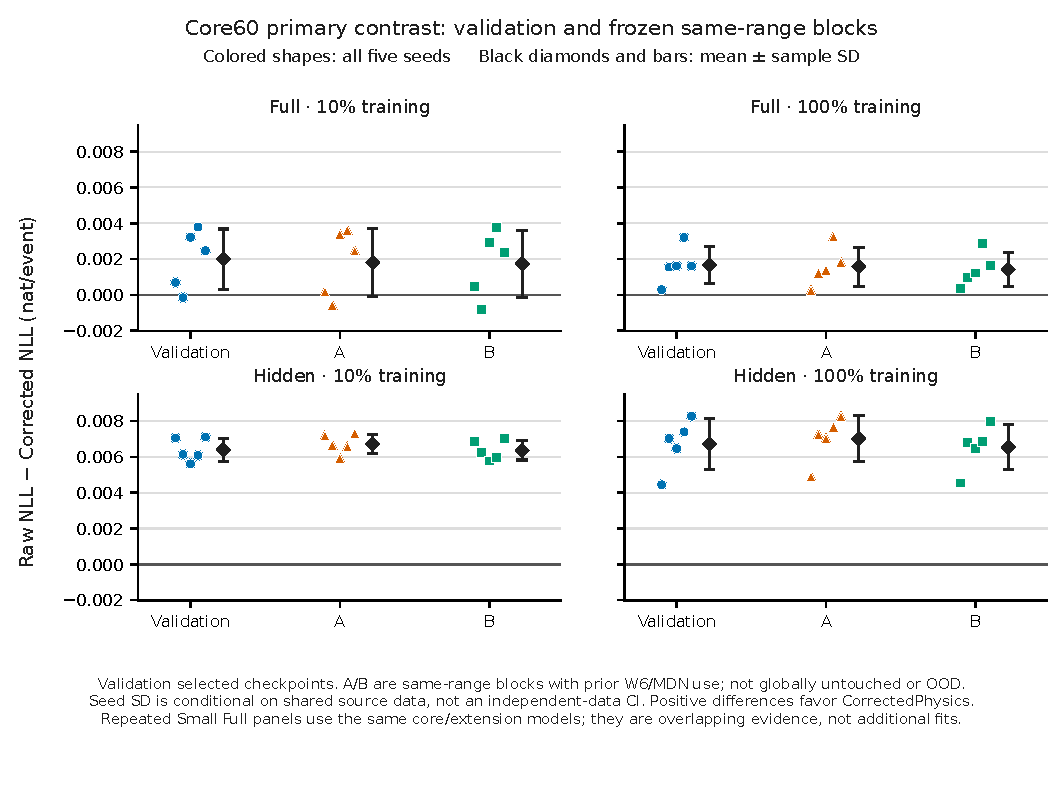
\includegraphics[width=\linewidth]{figures/correction_core_confirmation.pdf}
\caption{Core Raw-minus-Corrected contrasts on selected validation and frozen
A/B. All five seeds and sample SD are shown on one shared scale. Hidden's
larger overall mean gain does not imply better absolute NLL or improvement in
every conditional group. A/B retain legacy same-range provenance.}
\label{fig:corrected_core_confirmation}
\end{figure}

\subsection{Secondary comparisons: capacity, training fraction and fitted centers}
\label{sec:corrected_full_confirmation}

The expanded Full matrix places the physical center alongside two fitted
centers and varies model capacity and training fraction.
CorrectedPhysics has lower mean NLL than Raw in all six capacity/fraction
groups on A and separately on B. The gains range from $0.001341$ to
$0.002326$ nat/event on A and from $0.001231$ to $0.002265$ on B
(Figure~\ref{fig:corrected_full_confirmation}). The selected-validation range
is $0.001616$--$0.002393$ nat/event. The Small 10\% comparison includes one
negative seed on all three datasets; Small 30\% includes an additional
negative seed on A. These exceptions remain in the complete tables.

All six Learned-minus-Corrected mean contrasts are also positive on validation,
A and B. Conversely, all six Simple-minus-Raw mean contrasts are negative:
the simple fitted center improves on Raw in mean, so mean improvement over Raw
is not unique to the physical center. Individual seed exceptions include
Learned-minus-Corrected at Large 100\% on all three datasets and at Small
30\% on A. Appendix Table~\ref{tab:full-primary-complete} and the complete A/B
tables retain all prespecified contrasts rather than only favorable means.

\begin{figure}[t]
\centering
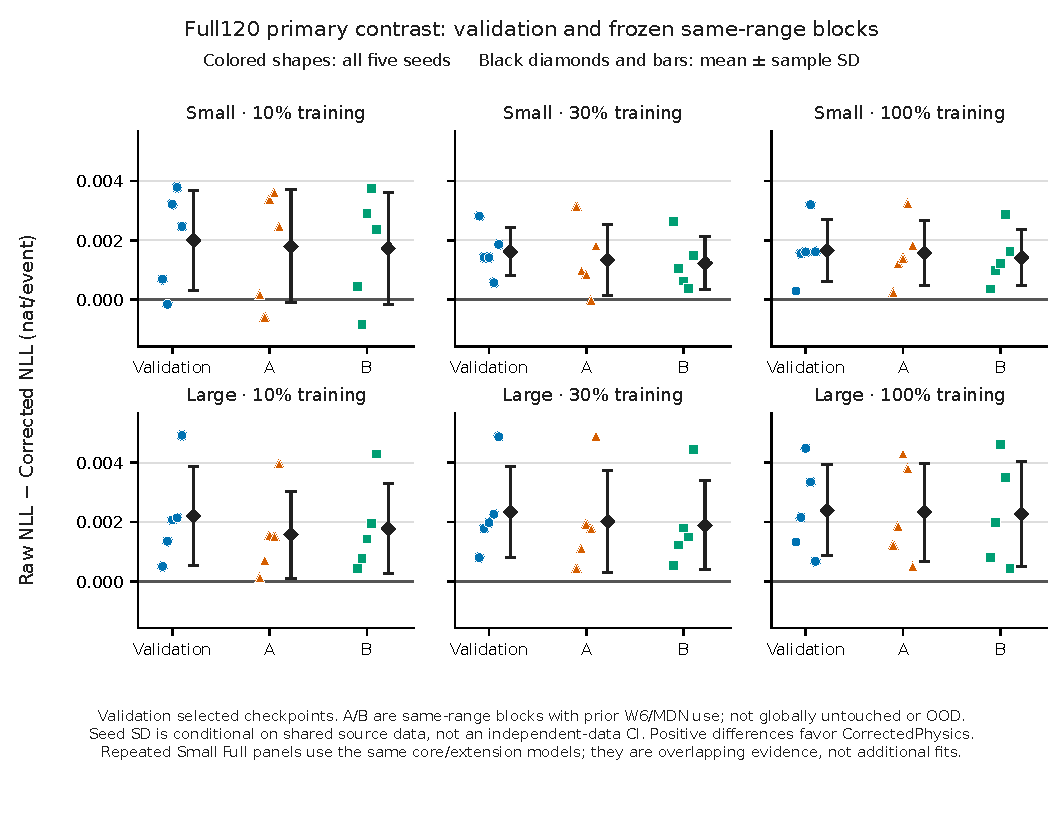
\includegraphics[width=\linewidth]{figures/correction_full_confirmation.pdf}
\caption{Full-conditioner Raw-minus-Corrected comparison at both capacities and
all three fractions. Negative seeds are retained. The Small Full 10\%/100\%
models overlap with the core figure and are not additional replications.
All other prespecified comparisons remain in the complete A/B tables.}
\label{fig:corrected_full_confirmation}
\end{figure}

Capacity and fraction effects are less consistent than the mean direction of
the representation comparison. The Small-minus-Large interaction of
Raw-minus-Corrected gains at 10\% changes mean sign between validation and A,
and is slightly negative on B. Fraction interactions also have mixed seed
directions. These results do not establish a monotonic capacity or sample-size
relationship under the fixed-update budget. An additional post-hoc comparison
of absolute NLL finds Small-minus-Large means below zero in all 36
representation/fraction/dataset groups. Thus a larger relative representation
gain at Large capacity does not identify the better absolute predictor in
this experiment.

\subsection{Post-hoc conditional performance: mean gains coexist with local losses}
\label{sec:local_results}

The 42 momentum--thickness--charge groups were fixed before scoring, but this
review of their heterogeneity was added after inspecting completed results.
It is descriptive and post-hoc. For each Hidden fraction on each block,
18 group means favor CorrectedPhysics and 24 favor Raw. The negative-mean
groups contain about 57.14\% of events; this is the event share of those bins,
not the fraction of individual events with worse likelihood. They occupy
momenta $[0.4,0.6)$ and $[0.8,1.0]$ GeV/$c$ across every thickness and charge.
The large event-weighted gain in $[0.3,0.4)$, about $0.086$--$0.094$ nat/event,
dominates the positive overall mean. Group means span approximately
$-0.048$ to $+0.123$ nat/event, and 12--13 groups have all five seed contrasts
negative. These observed bin means qualify the overall Hidden benefit. They do not,
by their count alone, establish a population-level regional failure pattern
or a significance claim. Conditional calibration is a separate property.

Each Full condition also has 2--9 negative group means, although none is negative
for every seed. All thickness-marginal means are positive, showing how a coarse
marginal can conceal momentum heterogeneity. These group counts are not
independent successful trials, and group means do not resolve within-bin behavior.

Table~\ref{tab:local_hidden} places the overall Hidden means alongside the
local contrast ranges. The repeated sign pattern across blocks and fractions
is a descriptive feature of these fixed bins, not an independent-bin test.

\begin{table}[t]
\centering
\caption{Post-hoc Hidden group summaries at Small capacity, in nat/event. A positive overall
Raw-minus-Corrected mean coexists with negative means in 24 of the 42
predefined groups. Ranges are across five-seed group means, not across events.
The last column counts groups in which all five seed contrasts are negative.}
\label{tab:local_hidden}
\small
\setlength{\tabcolsep}{4pt}
\begin{tabular}{llrrrr}
\toprule
Block & Fraction & \shortstack{Overall\\mean} & \shortstack{Negative\\groups} & Group mean range & \shortstack{All-five\\negative} \\
\midrule
A & 10\% & $+0.006720$ & 24/42 & $[-0.047278,+0.123132]$ & 13 \\
A & 100\% & $+0.007009$ & 24/42 & $[-0.041985,+0.117412]$ & 12 \\
B & 10\% & $+0.006372$ & 24/42 & $[-0.047979,+0.119093]$ & 12 \\
B & 100\% & $+0.006542$ & 24/42 & $[-0.042919,+0.116428]$ & 13 \\
\bottomrule
\end{tabular}
\end{table}

\subsection{Post-hoc location diagnostic and the erroneous-center control}
\label{sec:location_results}

The earlier matched 60-run comparison includes H to distinguish the intended physical
center from the earlier unit-inconsistent implementation. Under the same
controlled protocol, the source-validation Hidden Raw-minus-H means are
$-0.087870$ and $-0.087728$ nat/event at 10\% and 100\%, with every seed
negative. On A/B, the Hidden deficit remains approximately $0.088$ nat/event.
The unit-consistent center has the opposite mean direction, as reported in
Section~\ref{sec:conditioner_results}. This control establishes that the old
deficit does not characterize CorrectedPhysics; it was introduced after the
implementation error was identified, rather than as a planned physical
alternative in the original study.

Every representation separately fits $\mu=\operatorname{mean}_{\rm train}(Y-c)$.
Adding a constant to $c$ changes $\mu$ by the opposite constant; the standardized
residual and support coordinate absorb that offset. The amplitude of $c$ alone therefore does not predict a likelihood gain;
its variation across conditions must be considered after this offset is absorbed.

After viewing the validation results, we examined momentum-bin residual means
within each retained condition $W=(t,q)$ on the source diagnostic split. For
seven momentum bins $j$, with count $n_{jW}$ and residual mean $m_{jW}$, define
\begin{equation}
 N_W=\sum_j n_{jW},\quad
 m_W=\frac{\sum_j n_{jW}m_{jW}}{N_W},\quad
 v_W=\frac{\sum_j n_{jW}(m_{jW}-m_W)^2}{N_W}.
\end{equation}
The pooled metric is $[\sum_W N_W v_W/\sum_W N_W]^{1/2}$.
It is $8.01561\times10^{-6}$, $1.40700\times10^{-5}$ and
$5.88169\times10^{-6}$ GeV/c for Raw, H and CorrectedPhysics, respectively.
Both fractions give the same original-unit centered metric because the global
training mean cancels. This is variation of bin means, not within-bin event
variance; no confidence interval is estimated.

The global 42-bin location measure also contains between-thickness/charge
variation. H lowers that global measure while increasing the within-$W$
momentum measure, so the global measure must not be used as a Hidden-specific
burden. CorrectedPhysics lowers the within-$W$ metric. This post-hoc pattern is
consistent with the NLL directions but does not identify their unique cause:
finite-bin averaging, conditional shape/scale, support and optimization may
also contribute. The pooled diagnostic does not explain which individual
groups gain or lose likelihood.

\begin{figure}[t]
\centering
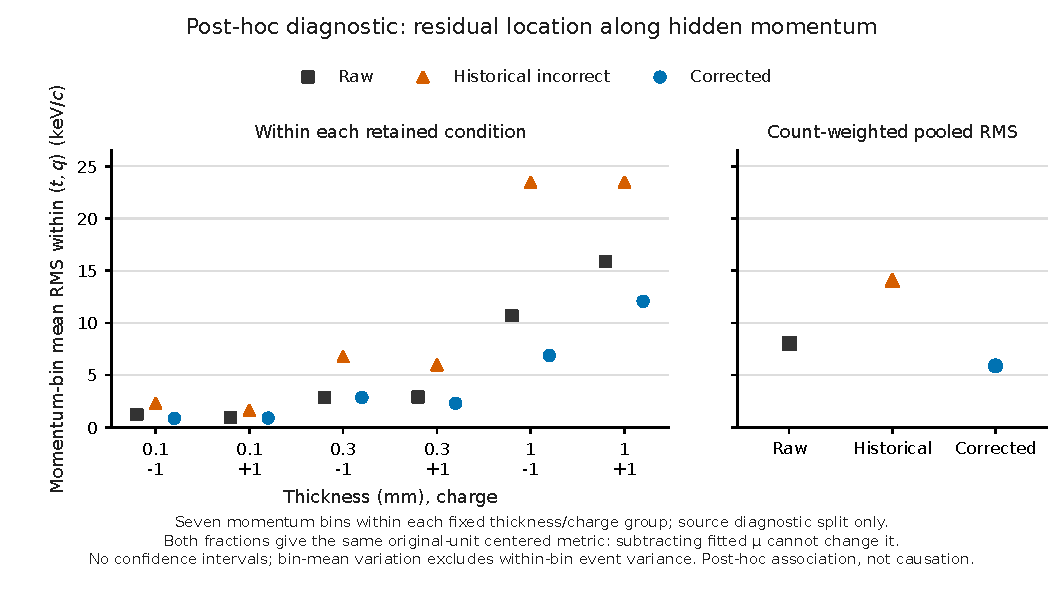
\includegraphics[width=0.95\linewidth]{figures/correction_within_condition.pdf}
\caption{Post-hoc residual-location diagnostic within fixed thickness and
charge. Every retained-condition group and the count-weighted pooled metric
are shown. Both fractions are retained in the source tables and coincide in
original units after centering. The plot contains no confidence intervals and
is neither a prespecified primary comparison nor causal identification.}
\label{fig:correction_location}
\end{figure}

